\snote{nested}

\subsection*{Motivation}

In the external validation the reduced model keeps the non-selected parameters at $\theta_0$, the published estimate, which was obtained from \emph{all} experimental data, including the test experiments. The reduced model may therefore inherit information about the test data through the parameters it keeps fixed. This note quantifies that effect.

\subsection*{Design}

For each problem we ran a \emph{nested} validation in which no value used by the reduced model has seen the test data:
\begin{enumerate}\itemsep0pt
  \item the full model was re-estimated on the training data only, giving $\hat\theta_{\mathrm{train}}$ (the full-model baseline of the external validation);
  \item the reduced model was then re-estimated on the training data with the non-selected parameters fixed at $\hat\theta_{\mathrm{train}}$ instead of $\theta_0$, and with search bounds derived from $\hat\theta_{\mathrm{train}}$;
  \item the test $\chi^2/n$ of this nested reduced model was compared with that of the full training fit and with that of the original, $\theta_0$-anchored reduced model.
\end{enumerate}
Twenty-nine problems were evaluated. Bertozzi (selected parameters active only in the test conditions), Blasi (single time point, no split) and Lang (277 free parameters, full re-estimation infeasible) were excluded. For Chen, whose full re-estimation with 155 free parameters did not finish in serial form, the columns of the finite-difference Jacobian were evaluated in parallel and the integrator tolerances were $10^{-6}/10^{-8}$; its $\theta_0$ and original values agree with those of the main analysis.

\subsection*{Results}

Supplementary Table~\ref{tab:nested} gives the results and Supplementary Figure~\ref{fig:anidada} compares them graphically.

\emph{The nested reduced model coincides with the full training fit.} In 19 of the 29 problems the two test values agree to better than 0.1\% and in 25 to better than 1\%. This agreement is expected by construction and is not evidence about leakage: the re-estimation of the reduced model starts at $\hat\theta_{\mathrm{train}}$, which already minimises the training error, so the optimiser has nothing to improve and returns essentially the full training fit. The exceptions are Schwen ($+248\%$, a worse local minimum of the two re-estimated parameters), Raia ($-5.1\%$), Chen ($-3.7\%$) and Brannmark ($+2.4\%$).

\emph{Removing the $\theta_0$ anchor removes the advantage of the reduced model.} Compared with the original reduced model, the nested reduced model predicted worse in 22 of the 29 problems and more than four times worse in eight (for example Brannmark 5.96 versus $6.4\times10^3$, Bruno 0.91 versus 208, Weber 1.00 versus 16.0, Zheng 1.58 versus 20.8). The better prediction of the reduced model on real data (main text, \emph{Prediction of held-out experiments}) therefore reflects the information in the published values at which the other parameters are fixed. This does not affect the admissibility of the subsets, which is a property of the model, not of the data, and it is why the comparison of prediction without leakage is made on synthetic data, where $\theta_0$ carries no information about the truth (\sref{synth}).

An earlier version of this note interpreted the agreement between the nested reduced model and the full training fit as evidence that the anchor does not affect the conclusion; as explained above, that agreement holds by construction, and the comparison with the original reduced model shows the opposite.

{\small
\begin{longtable}{@{}lrrrrrr@{}}
\caption{Leakage-free nested validation (29 problems). $\chi^2_{\mathrm{orig}}$: reduced model with the non-selected parameters at $\theta_0$; $\chi^2_{\mathrm{full,train}}$: full model re-estimated on the training data; $\chi^2_{\mathrm{nested}}$: reduced model with the non-selected parameters at $\hat\theta_{\mathrm{train}}$; $\theta_0$: published estimate. $\Delta$\%: nested relative to full; last column: nested over original (above 1, the nested reduced model predicts worse).}\label{tab:nested}\\
\toprule
Problem & $\chi^2_{\mathrm{orig}}$ & $\chi^2_{\mathrm{full,train}}$ & $\chi^2_{\mathrm{nested}}$ & $\theta_0$ & $\Delta$\% & nested/orig \\
\midrule
\endfirsthead
\multicolumn{7}{@{}l}{\emph{(continued)}}\\
\toprule
Problem & $\chi^2_{\mathrm{orig}}$ & $\chi^2_{\mathrm{full,train}}$ & $\chi^2_{\mathrm{nested}}$ & $\theta_0$ & $\Delta$\% & nested/orig \\
\midrule
\endhead
Alkan & 2.75 & 3.37 & 3.37 & 2.47 & +0.0 & 1.23 \\
Armistead & 1.22 & 1.37 & 1.37 & 1.16 & -0.0 & 1.13 \\
Bachmann & 4.77 & 7.35 & 7.36 & 1.05 & +0.1 & 1.54 \\
Boehm & 2.57 & 11.2 & 11.2 & 0.341 & +0.0 & 4.37 \\
Borghans & 0.743 & 0.744 & 0.744 & 0.74 & +0.0 & 1.00 \\
Brannmark & 5.96 & 6,277 & 6,431 & 0.938 & +2.4 & 1079.76 \\
Bruno & 0.909 & 208 & 208 & 0.909 & +0.0 & 228.69 \\
Chen$^\dagger$ & 20.9 & 17.7 & 17.1 & 15.2 & -3.7 & 0.82 \\
Elowitz & 1.5 & 3.89 & 3.89 & 1.38 & -0.0 & 2.59 \\
Fiedler & 11.2 & 9.32 & 9.3 & 1.22 & -0.2 & 0.83 \\
Fujita & 5.94 & 8.03 & 8.03 & 5.63 & +0.0 & 1.35 \\
Giordano & $1.0\times10^{-7}$ & 0.00773 & 0.00773 & $7.4\times10^{-9}$ & +0.0 & 75542.33 \\
Isensee & 1.08 & 1.08 & 1.08 & 1.04 & -0.0 & 0.99 \\
Laske & 0.758 & 1.87 & 1.87 & 0.445 & +0.0 & 2.47 \\
Liu & 0.954 & 1.02 & 1.02 & 0.942 & -0.0 & 1.07 \\
Lucarelli & 1.66 & 3.34 & 3.35 & 1.02 & +0.1 & 2.02 \\
Okuonghae & $4.7\times10^{4}$ & $1.2\times10^{5}$ & $1.2\times10^{5}$ & $2.9\times10^{4}$ & -0.0 & 2.62 \\
Oliveira & 912 & $8.1\times10^{4}$ & $8.1\times10^{4}$ & $4.6\times10^{5}$ & +0.0 & 89.16 \\
Perelson & $4.0\times10^{-13}$ & $4.0\times10^{-13}$ & $4.0\times10^{-13}$ & $4.0\times10^{-13}$ & +0.0 & 1.00 \\
Rahman & 0.00199 & 0.0257 & 0.0257 & 0.00148 & +0.0 & 12.90 \\
Raia & 8.22 & 5.1 & 4.84 & 0.417 & -5.1 & 0.59 \\
Raimundez & 1.17 & 1.43 & 1.43 & 0.98 & +0.1 & 1.23 \\
Salazar-Cavazos & 102 & 124 & 124 & 96.9 & +0.0 & 1.22 \\
Schwen & 8.2 & 8.4 & 29.3 & 0.768 & +248.4 & 3.57 \\
Smith & $1.5\times10^{4}$ & $1.5\times10^{4}$ & $1.5\times10^{4}$ & $8.3\times10^{4}$ & -0.3 & 1.00 \\
Sneyd & 2.22 & 2.56 & 2.56 & 1.37 & -0.0 & 1.15 \\
Weber & 1 & 16 & 16 & 0.993 & +0.1 & 15.96 \\
Zhao & 0.345 & 0.345 & 0.345 & 0.345 & +0.0 & 1.00 \\
Zheng & 1.58 & 20.8 & 20.8 & 1.51 & +0.0 & 13.16 \\
\bottomrule
\end{longtable}
\vspace{-0.6\baselineskip}{\footnotesize $^\dagger$Chen: full-model re-estimation with the finite-difference Jacobian evaluated in parallel and integrator tolerances $10^{-6}/10^{-8}$.}\par

}

\begin{figure}[H]
\centering
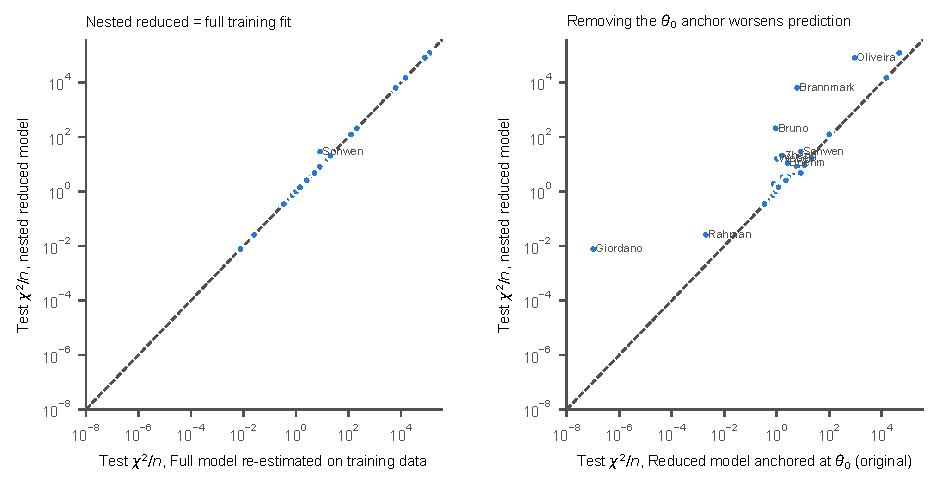
\includegraphics[width=\textwidth]{figures/figS_anidada.pdf}
\caption{\textbf{Leakage-free nested validation.} Test $\chi^2/n$ of the nested reduced model (non-selected parameters at $\hat\theta_{\mathrm{train}}$) against \textbf{a}, the full model re-estimated on the training data, with which it coincides by construction, and \textbf{b}, the original reduced model anchored at $\theta_0$; points above the diagonal predict worse without the anchor. Dashed line, $y=x$; problems that differ by more than a factor of 3 are labelled; Perelson ($\chi^2/n<10^{-12}$) lies outside the axes.}
\label{fig:anidada}
\end{figure}
